\chapter{Comportamiento SiguePersona visual con Drone real}\label{cap.real}
En este capítulo se explica lo que se ha desarrollado para conseguir un comportamiento sigue persona con un drone real con el objetivo de ser incluido en la plataforma \textit{Kibotics} para enseñanza de robótica.

Para ello se ha tenido que perfeccionar el driver aportado por el fabricante\cite{tellodriver}. Además como va a ser usado por niños, se ha tenido que hacer más amigable el interfaz, por ejemplo, en vez de tener que programar la detección de un objeto de un color indicado, se ha creado un método que recibe como parámetro el nombre del color y devuelve el cuadro que rodea dicho objeto.

\section{Diseño}
La aplicación desarrollada se compone de 2 partes claras (figura \ref{fig:esquemaReal}), la primera es la detección neuronal y la segunda los controladores PID.
\begin{figure}[H]
  \begin{center}
    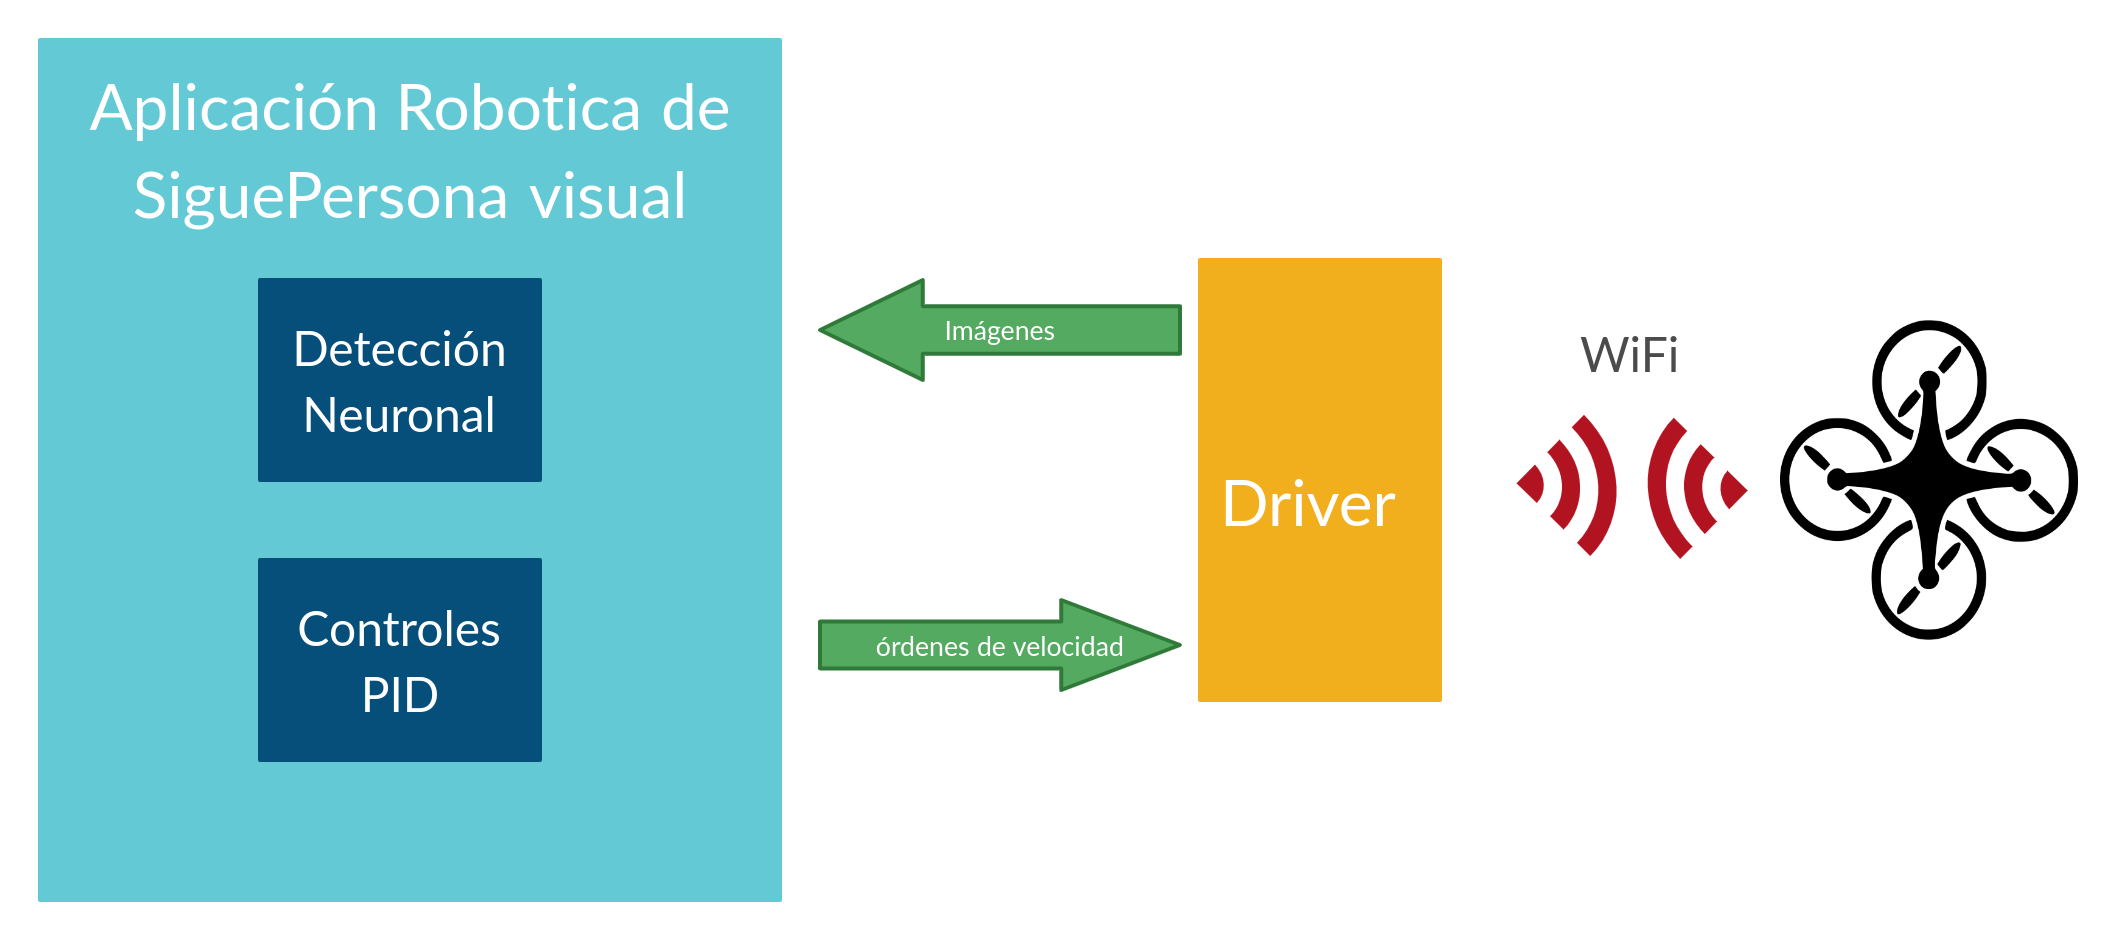
\includegraphics[width=0.7\textwidth]{figures/real/esquema.png}
		\caption{Diseño Aplicación}
		\label{fig:esquemaReal}
		\end{center}
\end{figure}

La detección neuronal es un recubrimiento de la red neuronal que recibe las imágenes del driver y devuelve los \textit{bounding boxes}, puntuaciones y clases detectadas. 
La parte de los controladores usando los \textit{bounding boxes} calcula la velocidades y se las pasa al driver.
\section{Desarrollo del \textit{driver}}
El \textit{driver} desarrollado para la plataforma \textbf{Kibotics} parte del proporcionado por el fabricante del drone. Añadiendo una serie de cambios por las limitaciones detectadas, además de necesitar simplificar el uso ya que está orientado a enseñanza infantil. 

Este \textit{driver} permite recibir imágenes de la cámara del drone, informaciones básicas como batería restante o tiempo de vuelo. Además permite controlar el drone tanto en velocidad, como en posición (avanza x metros, gira x grados,...),... 
\subsection{Primera versión}
Esta primera versión tiene el objetivo de subsanar los siguientes problemas:
\begin{itemize}
  \item El \textit{driver} no tiene control en velocidad.
  \item Si pasan 5 segundos sin recibir mensajes el drone se desactiva
  \item Las velocidades de entrada están en \textbf{cm/s} y \textbf{grados/s}.
\end{itemize}

\subsubsection*{No tiene control en velocidad}
El \textit{driver} aportado por el fabricante en \textit{Python} viene sin control en velocidad, si trae opciones para poder dar valor a las velocidades usadas por el drone y control en posición, pero no control en velocidad.
Después de analizar el documento del \acrshort{sdk}\footnote{\url{https://terra-1-g.djicdn.com/2d4dce68897a46b19fc717f3576b7c6a/Tello\%20\%E7\%BC\%96\%E7\%A8\%8B\%E7\%9B\%B8\%E5\%85\%B3/For\%20Tello/Tello\%20SDK\%20Documentation\%20EN_1.3_1122.pdf}} se vio que si existe un comando para el control en velocidad, pero que no se ha implementado en el driver aportado. 
Se implementa dicho método en el \textit{driver}. Además se implementa un hilo que se encarga de enviar cada poco tiempo la velocidad (500ms) como recordatorio porque, si no, como mecanismo de seguridad el drone se detiene si no recibe más mensajes de velocidad.

\subsubsection*{Las velocidades de entrada están en \textbf{cm/s} y \textbf{grados/s}}
La intención ha sido que se use el sistema internacional en todo momento y en este caso son \textbf{m/s} y \textbf{rad/s}.
Esto es tan fácil como realizar las conversiones pertinentes en las funciones para establecer las velocidades.

\subsubsection*{Si pasan 5 segundos sin recibir mensajes el drone se desactiva}
Este problema ha sido abordado añadiendo un hilo de \textbf{Python}(perro de guarda, \textit{watchdog}) que se encargue se enviar velocidades cada \textbf{500ms}. De esta manera evitamos que el \textit{Drone} se desactive.

\subsection{Segunda versión}
Los problemas subsanados en esta versión han sido los siguientes:
\begin{itemize}
  \item \textit{Driver} necesario en \textbf{Python 3.x} pero está escrito en \textbf{Python 2.7}. 
  \item Poca fiabilidad en el envío de mensajes del \textit{driver} al drone.
  \item El control en velocidad es poco reactivo.
\end{itemize}
\subsubsection*{Convertir el \textbf{driver} de Python 2.7 a Python 3.x}
Esto ha sido fácil porque casi todo el código de la aplicación funcionaba en\textbf{ Python 3}, las únicas diferencias eran la manera de importar los módulos que varía de entre las dos versiones y que en \textbf{Python 2} los bytes se representan como cadenas de texto(\textit{String}) y en \textbf{Python 3} son del tipo bytes.
\begin{table}[H]
\centering
\begin{tabular}{|c|c|c|}
\hline
\textbf{Tipo de cambio}          & \textbf{Python 2} & \textbf{Python 3} \\ \hline
Representación de bytes          & ' '               & b' '              \\ \hline
Importar desde mismo repositorio & import module     & import .module    \\ \hline
\end{tabular}
\caption{Cambios de \textbf{Python 2} a \textbf{Python 3} efectuados}
\label{tab:cambios_python_2_3}
\end{table}

En la tabla \ref{tab:cambios_python_2_3} se pueden ver los cambios efectuados.

\subsubsection*{Poca fiabilidad en el envío de mensajes del \textit{driver} al drone}
La comunicación con el Drone consiste en enviar un mensaje y recibir una respuesta que indica que lo ha recibido, o en el caso de pedirle algún dato, como la batería restante el dato en si.

El problema radica en que en frecuentemente en la \textit{WiFi} que comunica drone y ordenador o se pierde el mensaje que se envía o  se pierde la respuesta. Por lo que se ha implementado un mecanismo de reenvío de mensajes. Si no se recibe respuesta se vuelve a enviar el mismo mensaje hasta tener respuesta o se alcance el número máximo de reintentos.

\subsubsection*{El control en velocidad es poco reactivo}
 Para mejorar este apartado solo ha hecho falta reducir el tiempo entre mensajes de velocidad a \textbf{25ms}. Además no importa que se pierdan mensajes porque enseguida se envía otro con la velocidad actualizada.

\section{Detección visual de la persona}
Para elegir la red se han comparado tres del conjunto de redes preentrenadas preentrenada con el \textit{dataset} \acrshort{coco} de \textit{Object Detection API}\footnote{https://github.com/tensorflow/models/blob/master/research/object_detection/g3doc/tf2_detection_zoo.md}:
\begin{itemize}
  \item SSD Mobilenet v2 FPN de 320x320
  \item CenterNet resnet50 FPN de 512x512
  \item SSD Resnet50 FPN de 640x640
\end{itemize}
Para esta elección se ha grabado un vídeo con la cámara del drone (en todo momento hay una persona) y se ha usado el mismo vídeo con las tres opciones, y en un ordenador con un procesador I7 de octava generación, 16 GB de RAM y con gráfica integrada, obteniendo los resultado de la tabla \ref{tab:comparativa_redes}.
\begin{table}[H]
\centering
\begin{tabular}{|c|c|c|c|}
\hline
\textbf{Red}          & \textbf{Tiempo} & \textbf{Detecciones} & \textbf{Score} \\ \hline 
SSD Mobilenet v2      & 90ms            & 79\%        & 64\%           \\ \hline  
SSD Resnet50 v1       & 240ms           & 86\%        & 71\%           \\\hline  
CenterNet Resnet50 v1 & 450ms           & 85\%        & 71\%           \\ \hline 
\end{tabular}
\caption{Comparativa de redes}
\label{tab:comparativa_redes}
\end{table}
Se ha elegido \textit{SSD Mobilenet v2 FPN}(figura \ref{fig:mobilenet}) porque es la única que funciona a una velocidad razonable.
\begin{figure}[H]
  \begin{center}
    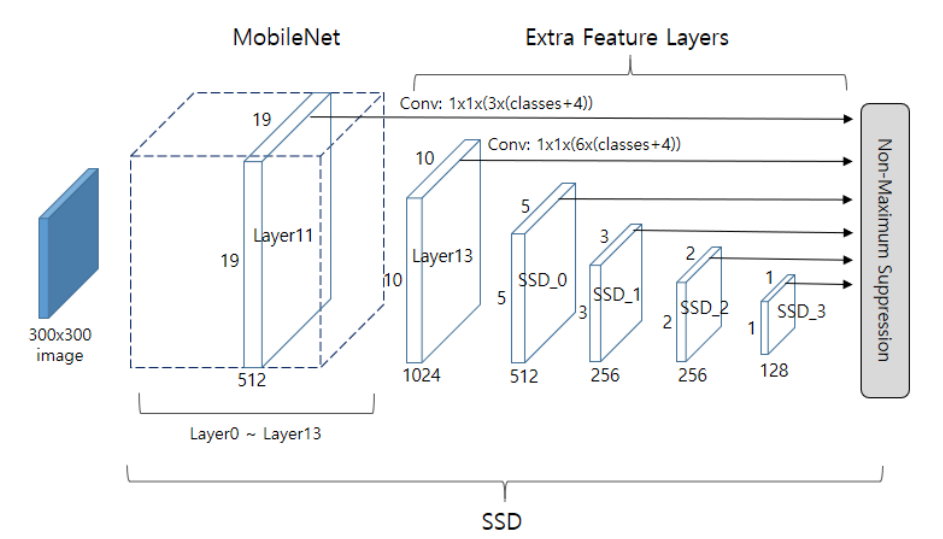
\includegraphics[width=0.6\textwidth]{figures/real/mobilenet.png}
		\caption{Esquema de una red Mobilenet ssd}
		\label{fig:mobilenet}
		\end{center}
\end{figure}
Esta red tiene 3 componentes principales: 
\begin{itemize}
  \item \textit{\gls{fpn} lite}\cite{fpn}. Permite extraer características de la imagen con indiferencia del tamaño del objeto 
  \item \textit{Mobilenet v2}\cite{mobilenetv2}. Es una red convolucional de extracción de características.
  \item \textit{\gls{ssd}\cite{ssd}}. Comprueba si hay cada clase en las regiones de interés seleccionadas y permite un mayor ajuste de dicha región.
\end{itemize}

Para poder trabajar con ella en se usa \textbf{Tensorflow 2.0}. Además se ha tenido que desarrollar un recubrimiento para poder usar la red de manera fácil.
Esta clase desarrollada permite cargar la red indicada por configuración ya sea un modelo de \textbf{Tensoflow} o un grafo. Además agrega un postprocesado de la información de salida de la red: 

\begin{itemize}
  \item convirtiendo en \textit{numpy arrays} los datos desde tensores
  \item Desechando los resultados con una puntuación menor al límite indicado por configuración.
  \item Filtrando los resultados para quedarse con las clases buscadas, en este caso personas.
  \item También se convierten los tamaños de las regiones de interés de porcentaje a píxeles.
\end{itemize}

Además se ha creado también otro nivel de abstracción superior para la fuente de la imagen para ayudar a su uso, así mediante configuración se indica si la fuente es el drone, una webcam, un directorio de imágenes o un vídeo y la fuente en sí y no hay que preocuparse de procesar la imagen para convertirla en RGB en caso de que sea la fuente no lo sea por ejemplo. La red recibirá siempre la imagen igual provenga del origen que provenga.

La red al final devuelve 3 \textit{arrays}, el primero con la clase a la que pertenecen las predicciones , el segundo con la regiones de interés o \textit{bounding boxes} (x mínima, y mínima, x máxima, y máxima) y el tercero con las puntuaciones.

\section{control PID}
El control PID es un bucle de control que calcula la siguiente operación en cada iteración.
\[ u(t) = K_p e(t) + K_i \int_{t}^{0} e(t') dt' + K_d \frac{de(t)}{dt}\]
Donde \textbf{e} es el error con respecto al objetivo y las \textbf{K} constantes que deben calcularse experimentalmente.

Una vez que se procesa la imagen recibida por el drone y se tienen las predicciones, se selecciona la persona con mayor puntuación y de su \textit{bounding box} se extrae posición central, el área y la posición superior.

Para controlar el drone se va a hacer con tres velocidades, avance, giro y movimiento vertical. Para ello se utiliza un control PID (en este caso debido al funcionamiento del drone solo proporcional y derivativo) para cada una de las velocidades.

En el caso de la velocidad de avance, se toma como referencia el área, para el giro la posición del centro en las coordenadas x de la imagen y para el la altura se usa la posición superior del \textit{bounding box}.
En el caso de la velocidad vertical se ha decidido usar como referencia la posición superior del \textit{bounding box} posicionándolo en torno a un 10\% de la parte superior de la imagen con el objetivo que se vea la cara de la persona. se probó también la manera fácil que es centrar verticalmente la persona en la imagen, pero puede ocurrir que solo se tenga una parte de la persona y esté centrado. como se puede ver en las imágenes \ref{fig:real1} y \ref{fig:real2} en ambos casos el centro del cuadrado está muy próximo al centro vertical de la imagen, pero no por ello estar bien.

\begin{figure}[!htb]
\minipage{0.45\textwidth}
    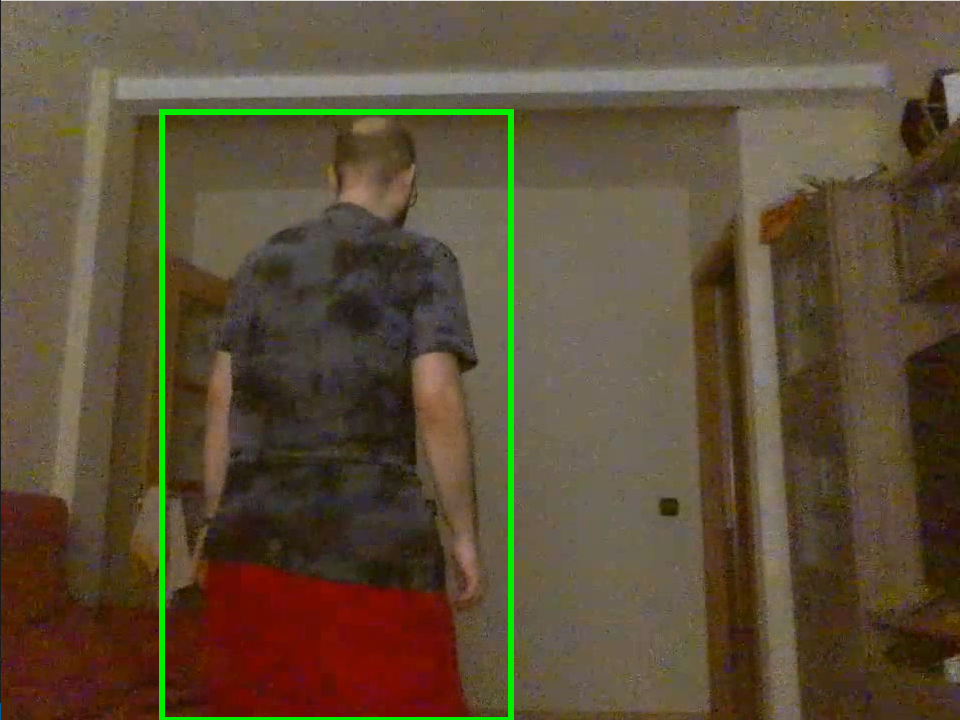
\includegraphics[width=\linewidth]{figures/real/cap1.png}
    \caption{Persona seleccionada}\label{fig:real1}
\endminipage\hfill
\minipage{0.45\textwidth}
    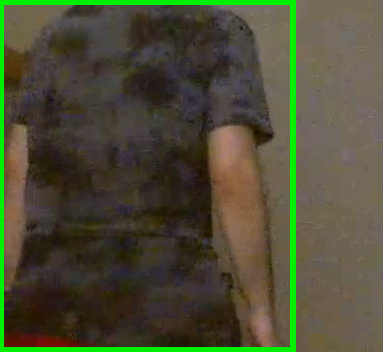
\includegraphics[width=\linewidth]{figures/real/cap2.png}
    \caption{Torso detectado}\label{fig:real2}
\endminipage\hfill
\end{figure}

En cambio tomando como referencia el punto más alto del cuadrado se tiende a obtener la imagen \ref{fig:real1} que además facilita la detección de la persona.
